	\begin{figure*}[t!]
	\begin{center}
		
		\begin{tabular}{@{}c@{~~}c@{~~}c@{~~~~}|@{~~~~}c@{}c@{~~}c@{}c@{~~}c@{}c@{}}
			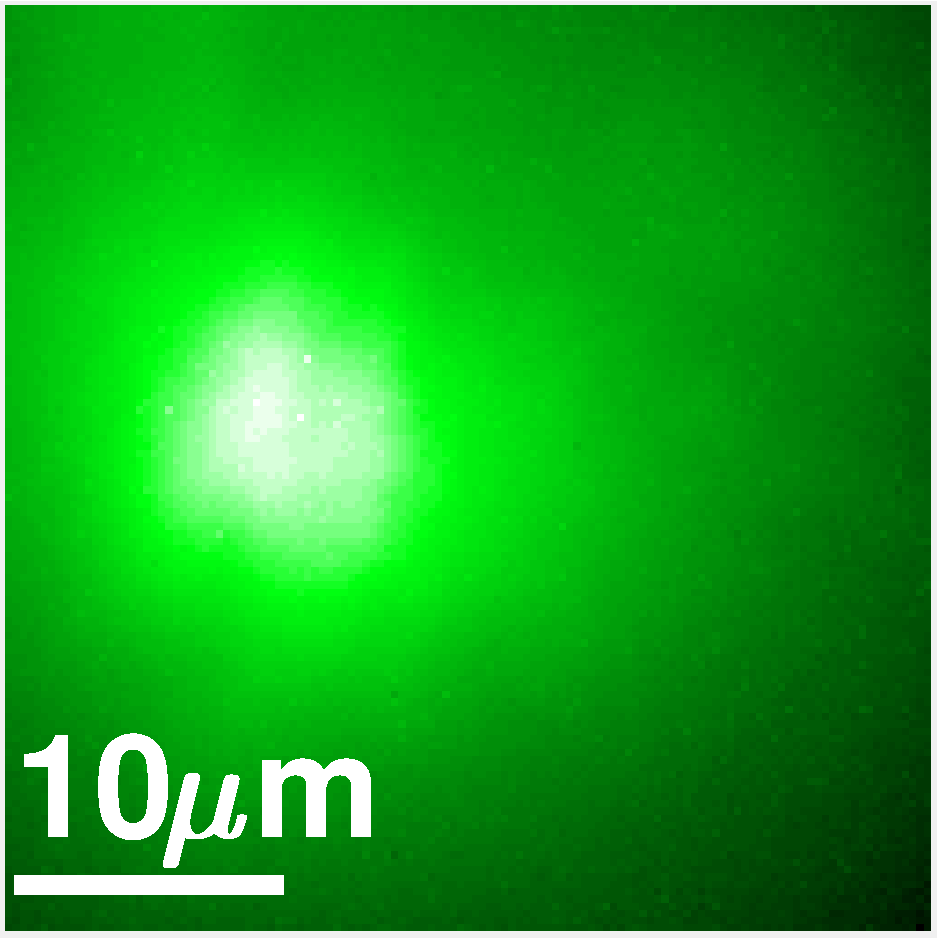
\includegraphics[width= 0.13\textwidth]{figs/confocal_res/fig_big_area/2023_06_08_18_48_03/1.pdf}&
			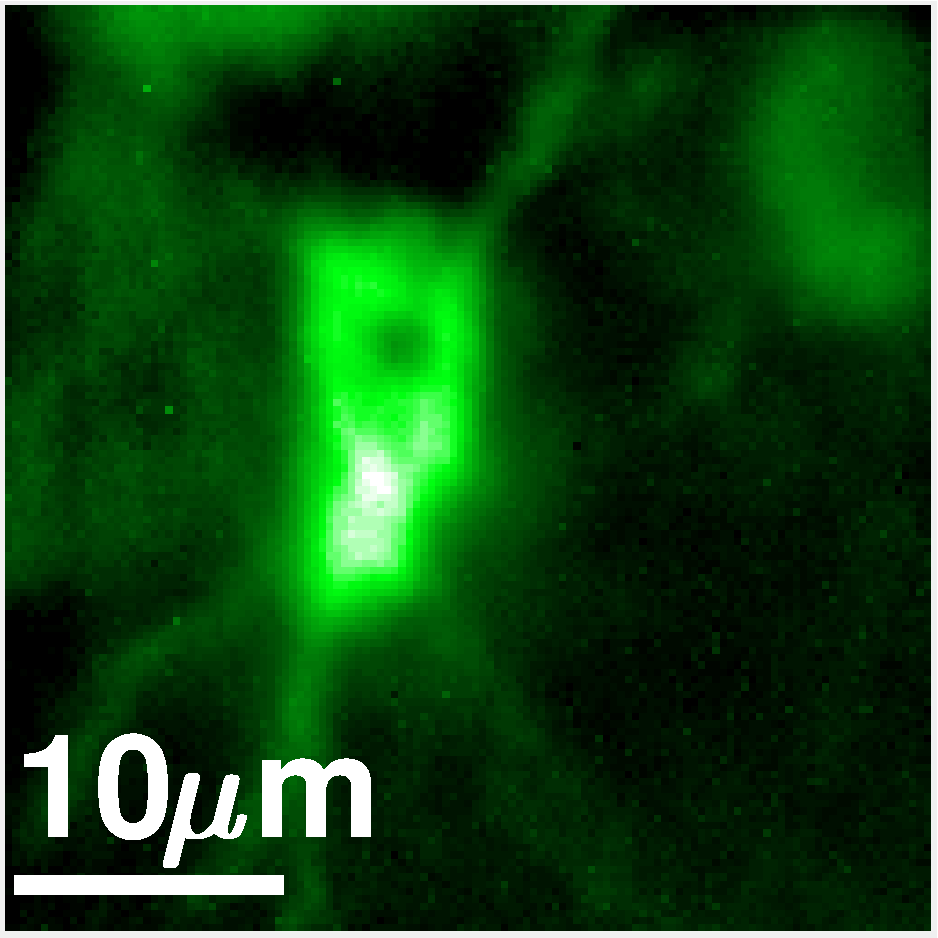
\includegraphics[width= 0.13\textwidth]{figs/confocal_res/fig_big_area/2023_06_08_18_48_03/2.pdf}&
			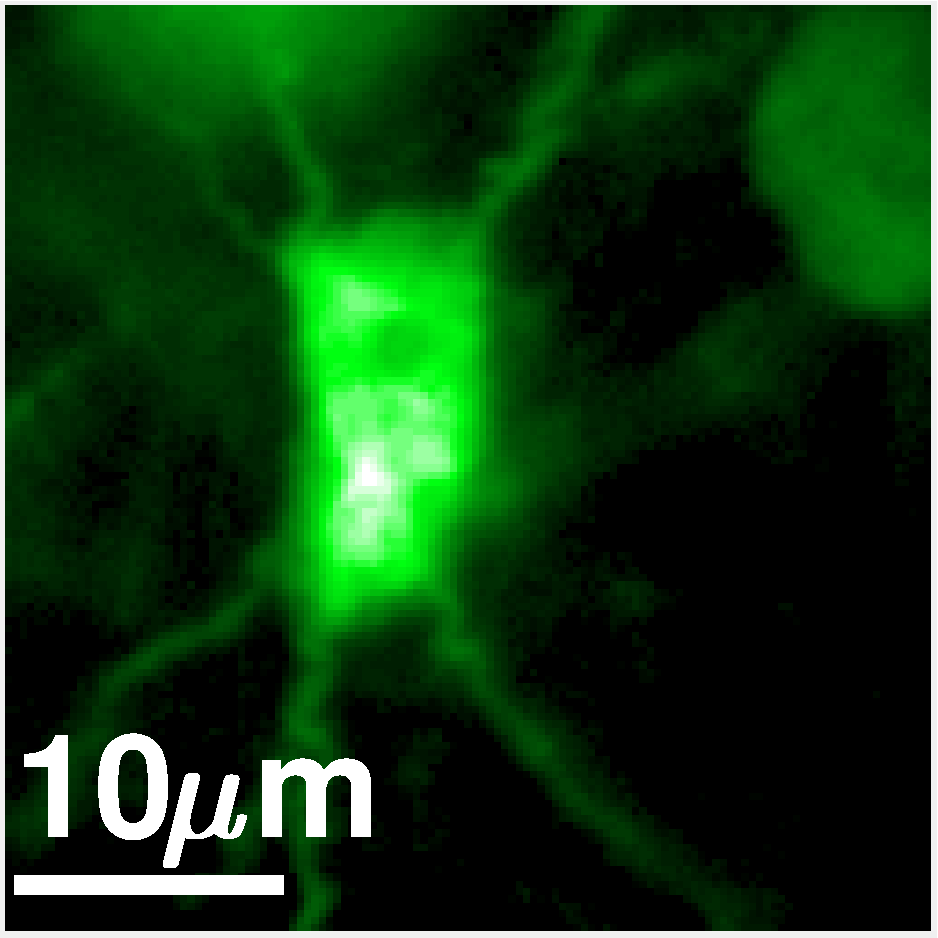
\includegraphics[width= 0.13\textwidth]{figs/confocal_res/fig_big_area/2023_06_08_18_48_03/3.pdf}&
		
			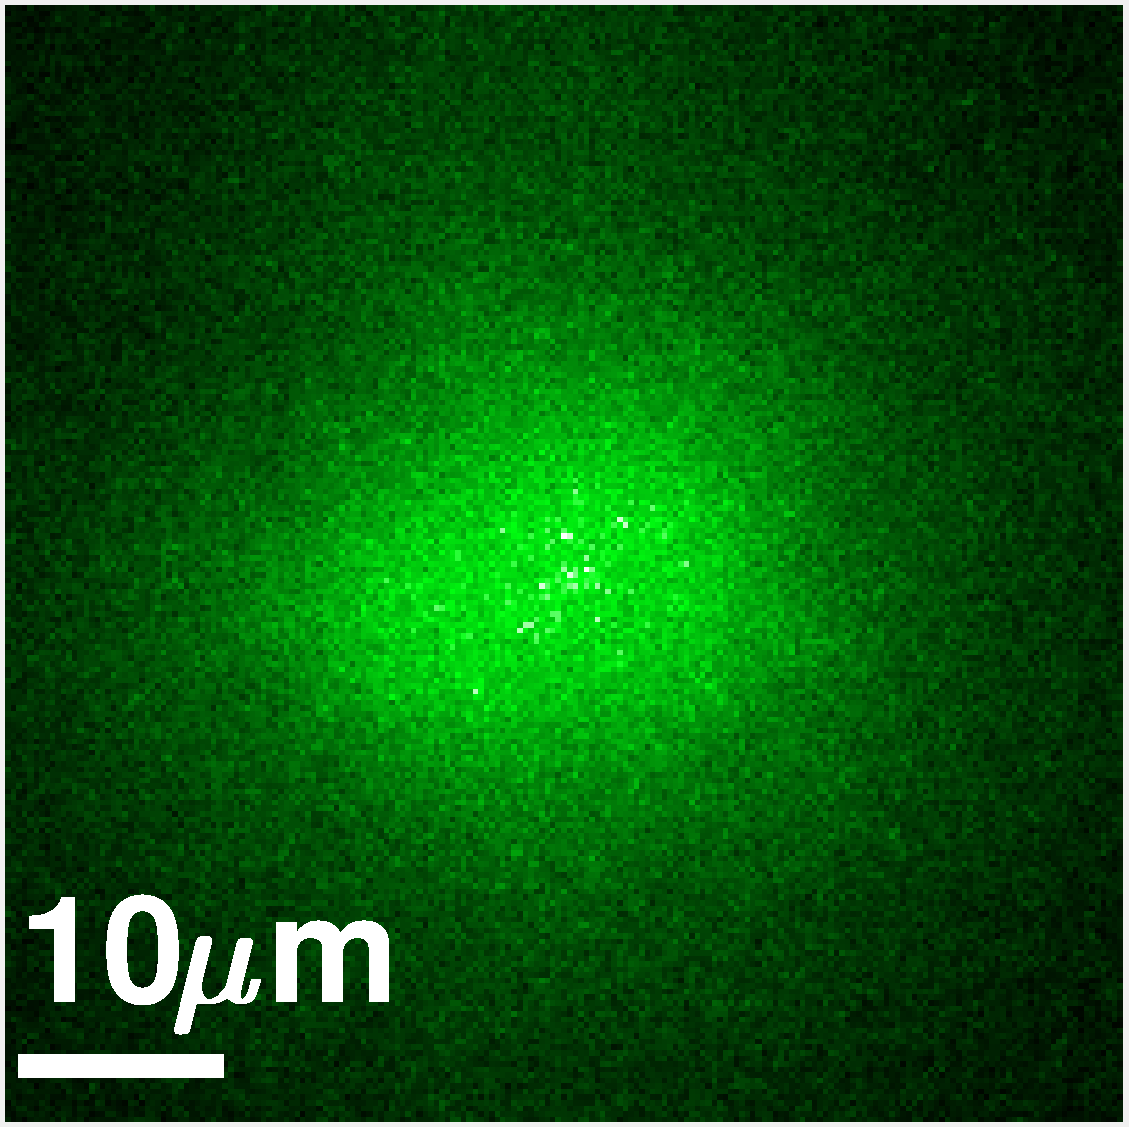
\includegraphics[width = 0.13\textwidth]{figs/confocal_res/fig_converging/2023_01_11_18_28_55/BSI_init.pdf}&
			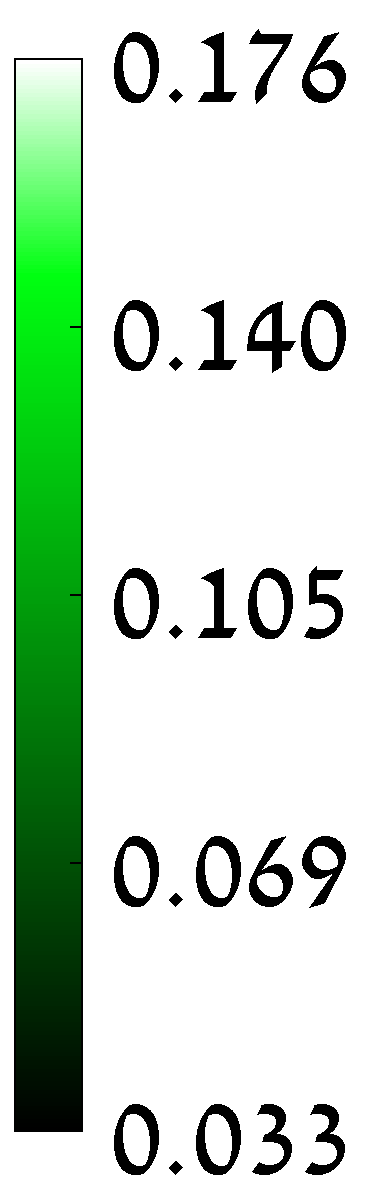
\includegraphics[height = 0.13\textwidth]{figs/confocal_res/fig_converging/2023_01_11_18_28_55/BSI_init_colorbar.pdf}&
			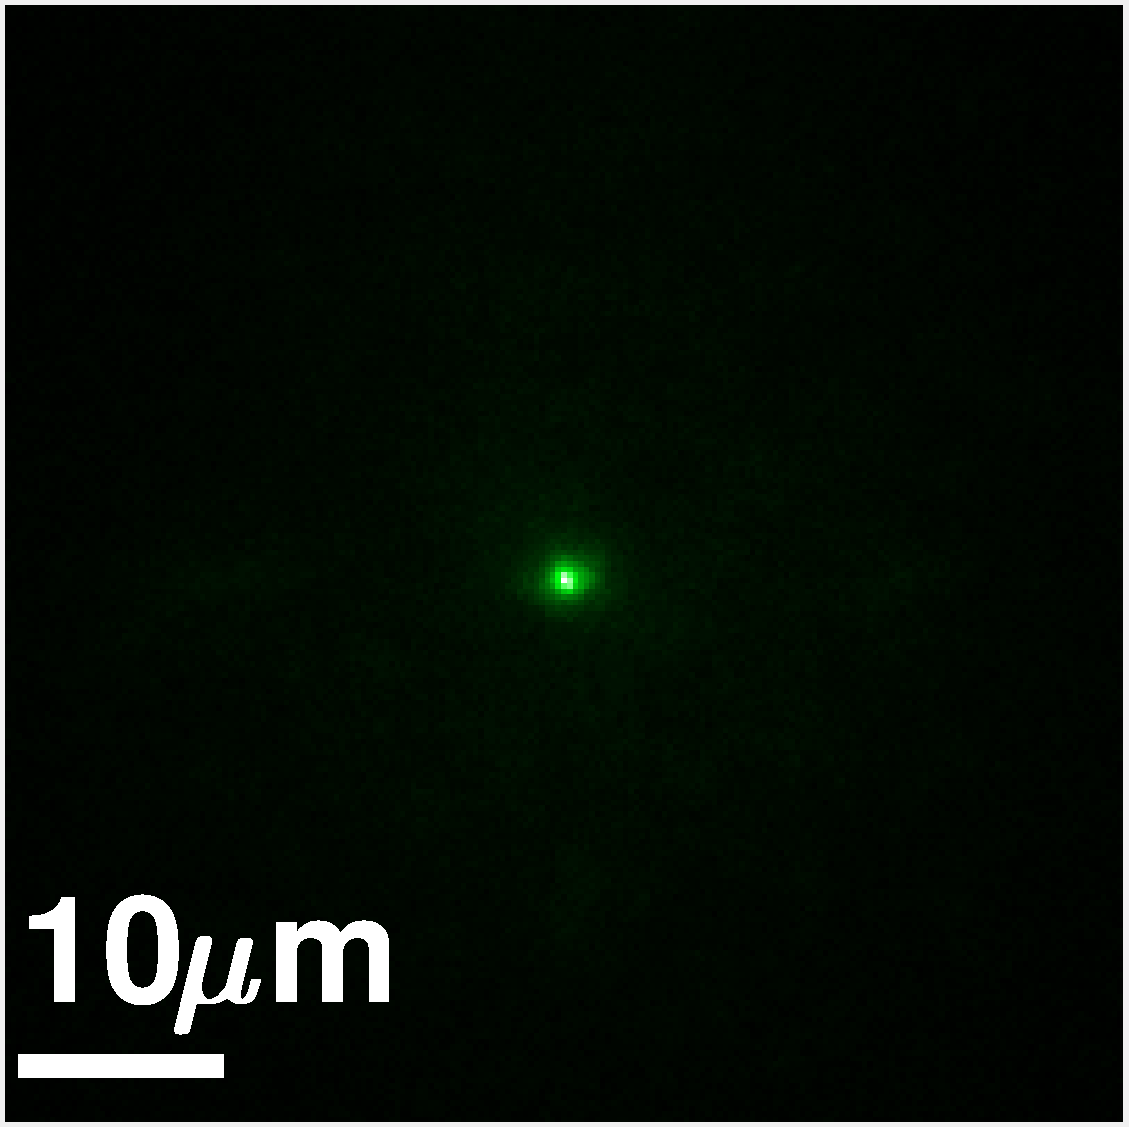
\includegraphics[width = 0.13\textwidth]{figs/confocal_res/fig_converging/2023_01_11_18_28_55/BSI_fin.pdf}&
			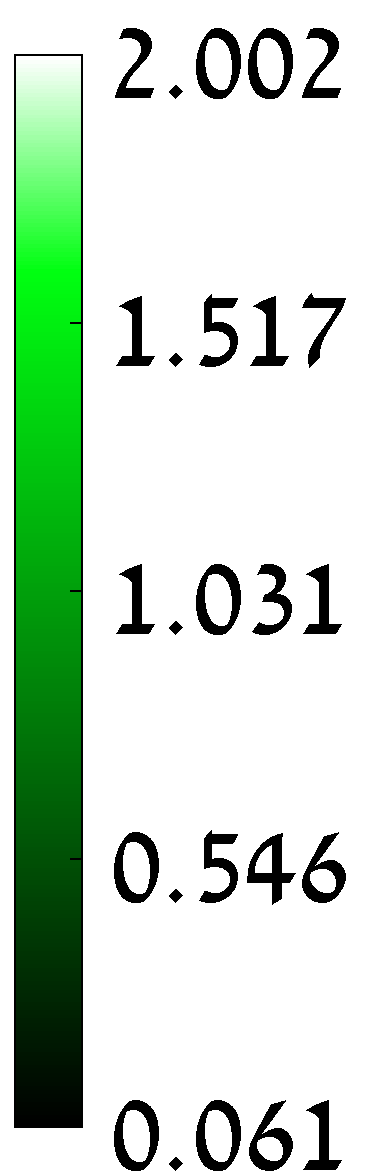
\includegraphics[height = 0.13\textwidth]{figs/confocal_res/fig_converging/2023_01_11_18_28_55/BSI_fin_colorbar.pdf}&
			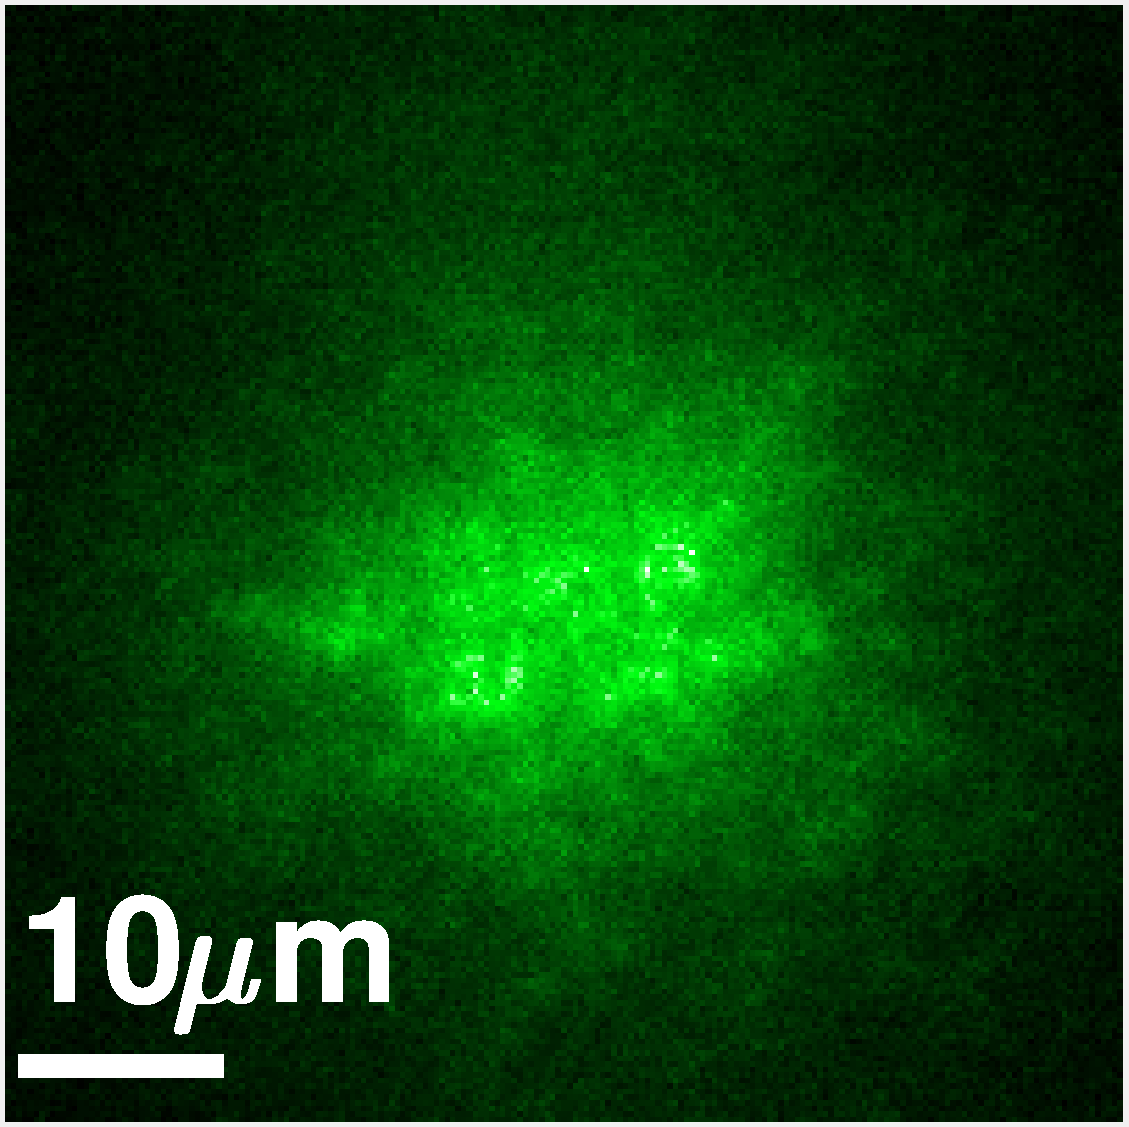
\includegraphics[width = 0.13\textwidth]{figs/confocal_res/fig_converging/2023_01_11_18_28_55/BSI_fin_psf.pdf}&
			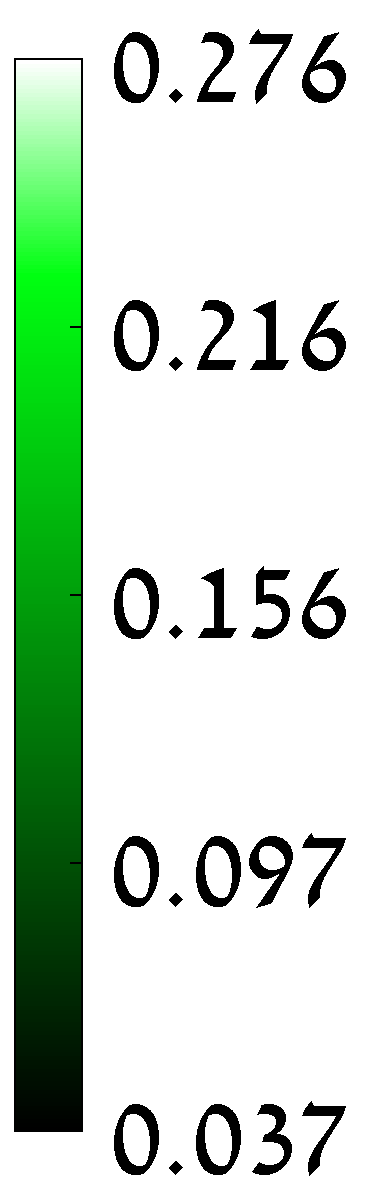
\includegraphics[height = 0.13\textwidth]{figs/confocal_res/fig_converging/2023_01_11_18_28_55/BSI_fin_psf_colorbar.pdf}\\
			
			
			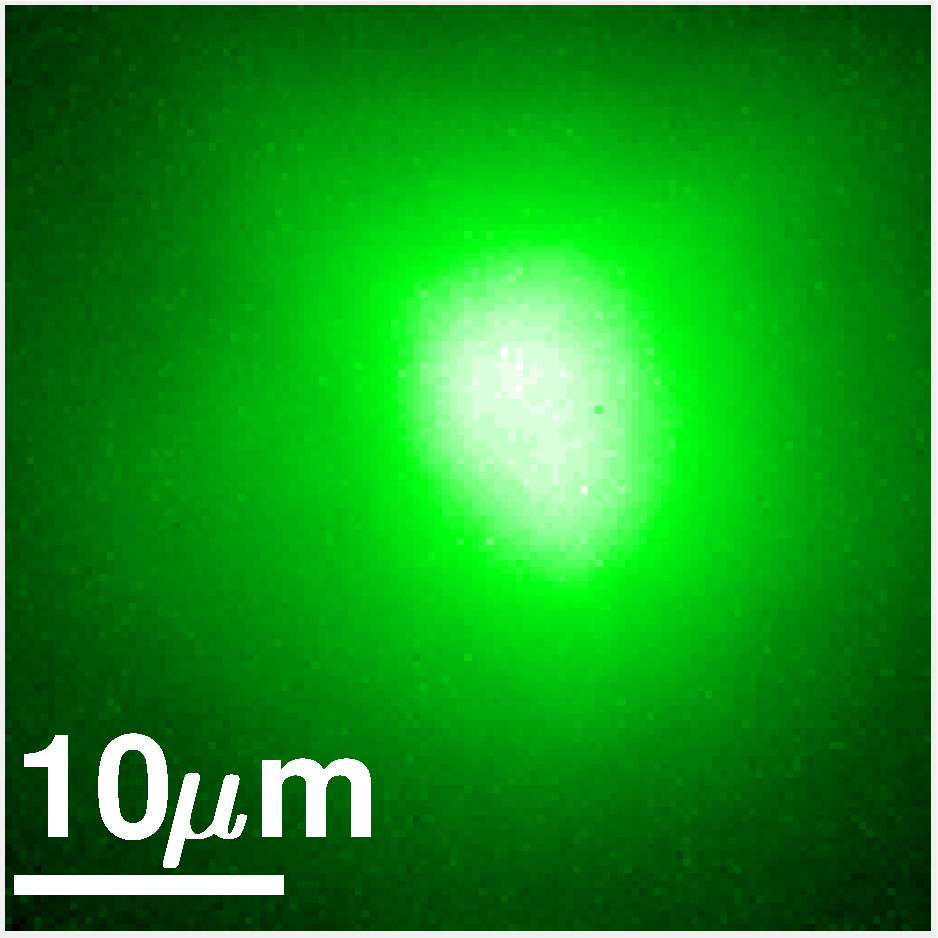
\includegraphics[width= 0.13\textwidth]{figs/confocal_res/fig_big_area/2023_06_05_15_57_55/1.pdf}&
	    	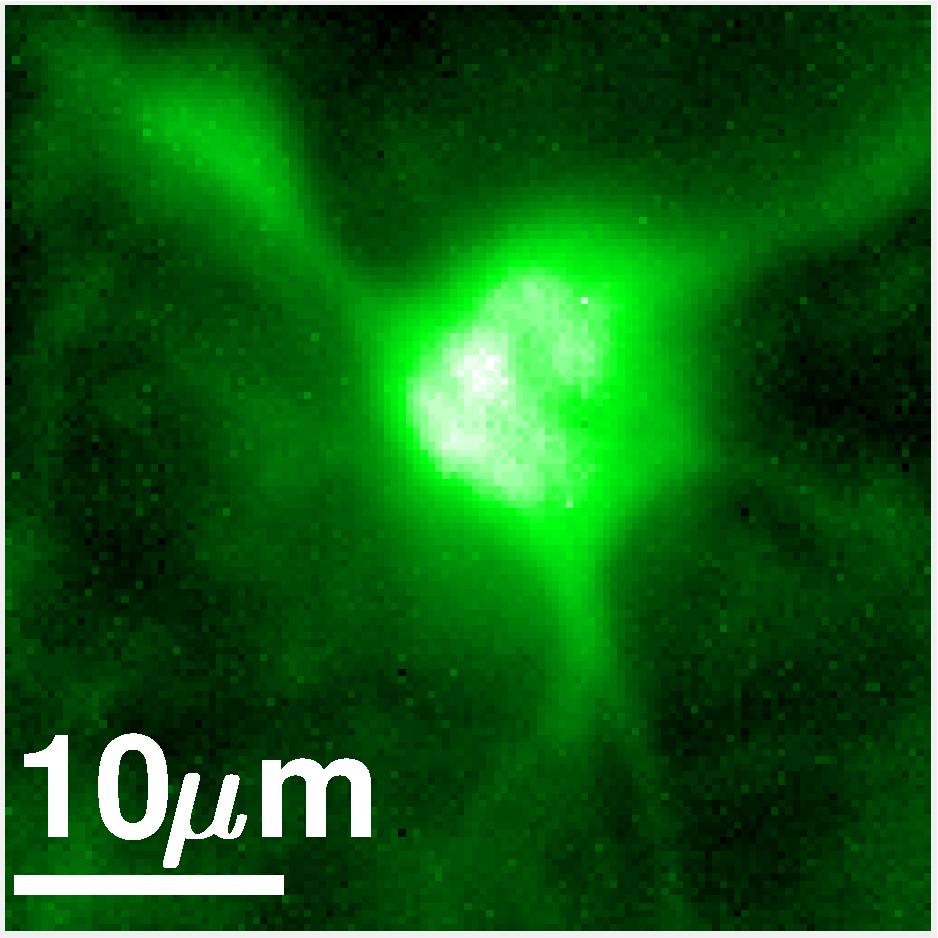
\includegraphics[width= 0.13\textwidth]{figs/confocal_res/fig_big_area/2023_06_05_15_57_55/2.pdf}&
	    	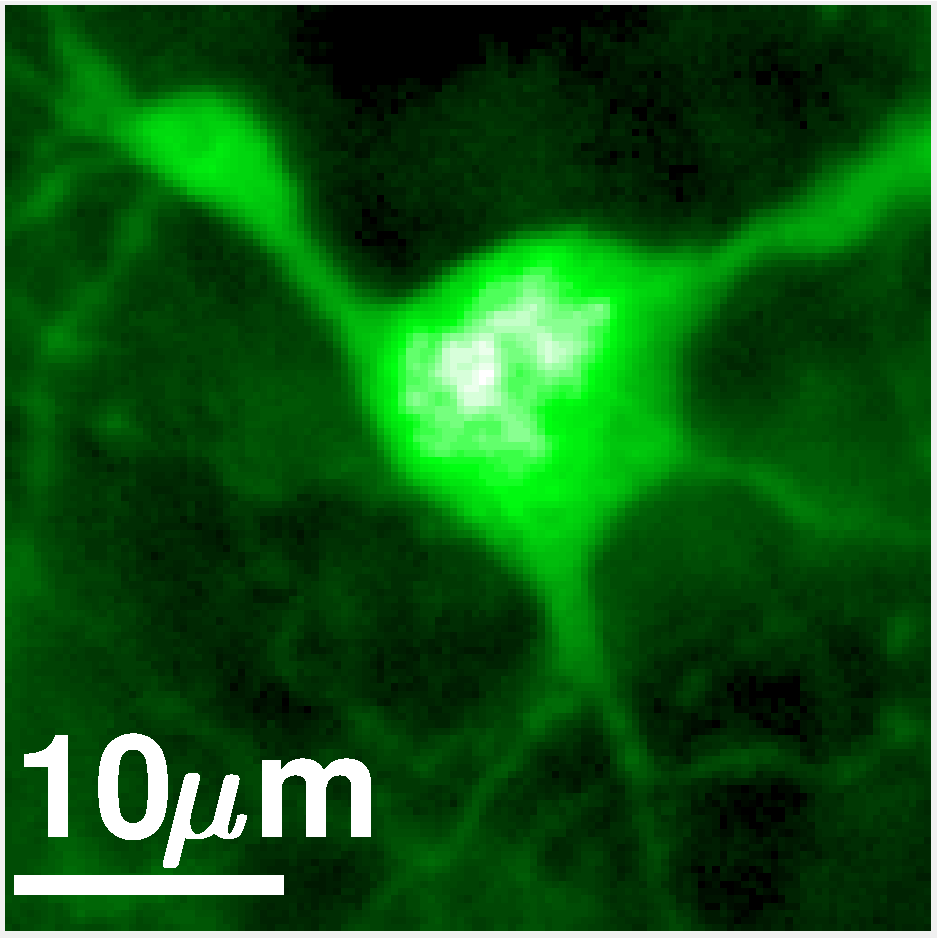
\includegraphics[width= 0.13\textwidth]{figs/confocal_res/fig_big_area/2023_06_05_15_57_55/3.pdf}&
		
			
			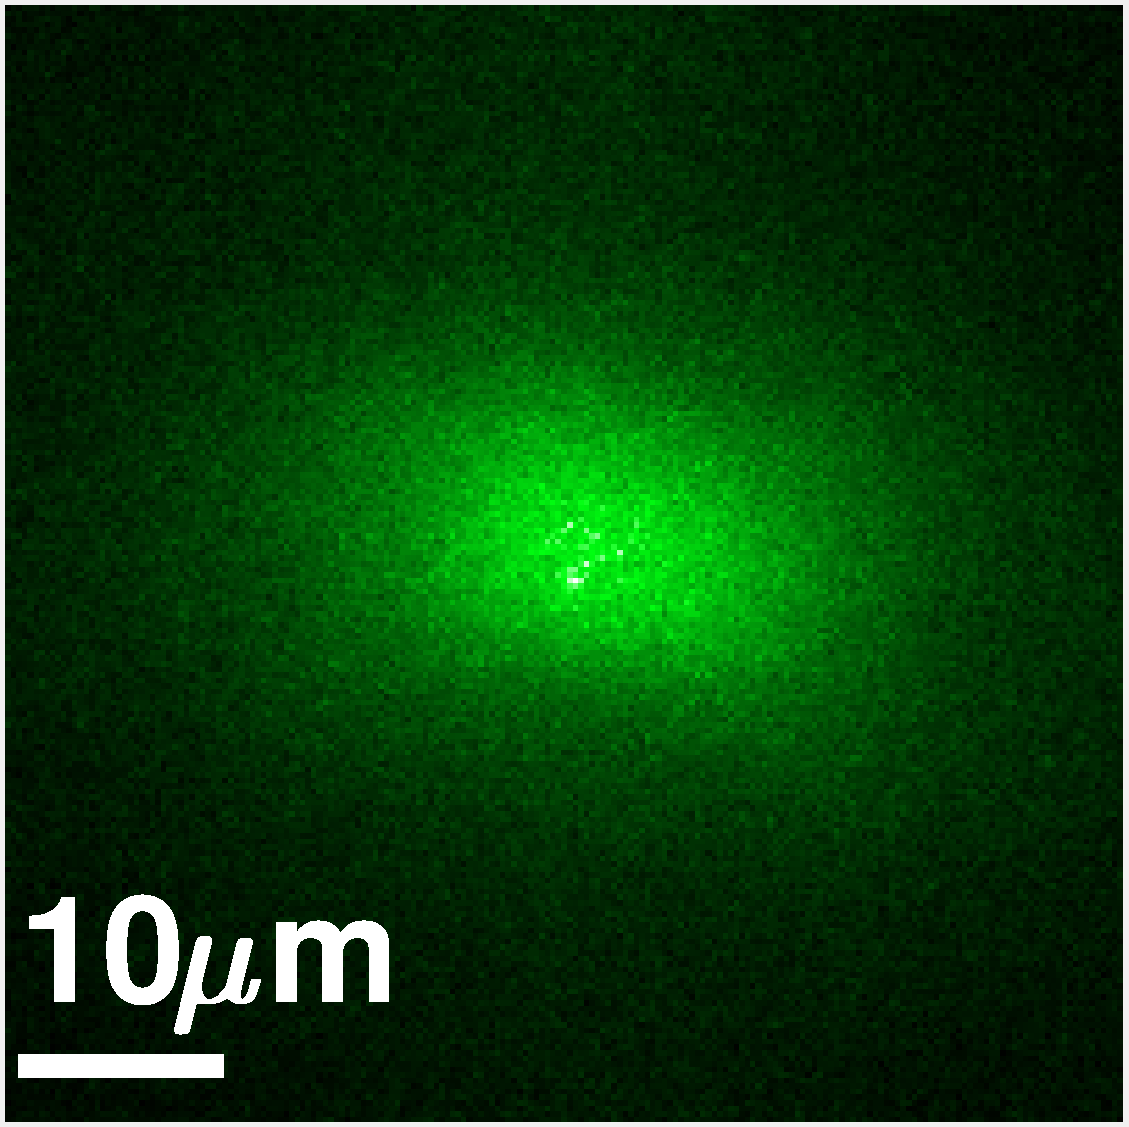
\includegraphics[width = 0.13\textwidth]{figs/confocal_res/fig_converging/2023_01_10_17_18_44/BSI_init.pdf}&
			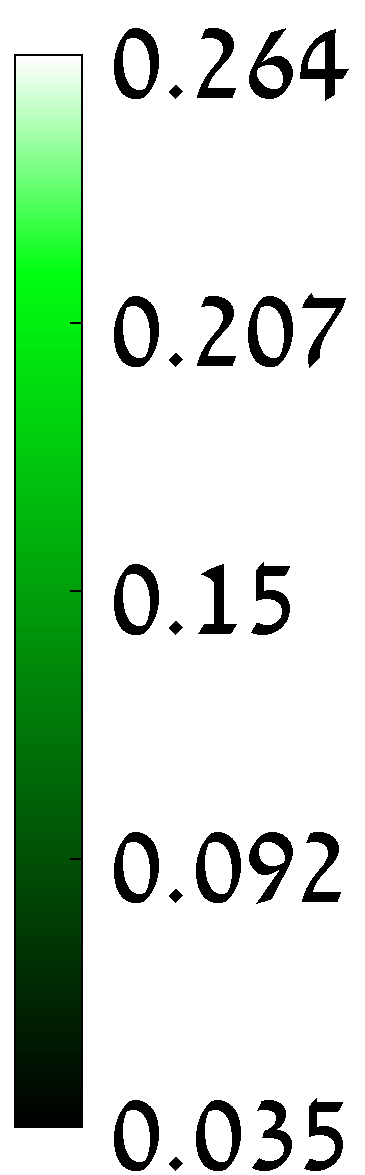
\includegraphics[height = 0.13\textwidth]{figs/confocal_res/fig_converging/2023_01_10_17_18_44/BSI_init_colorbar.pdf}&
			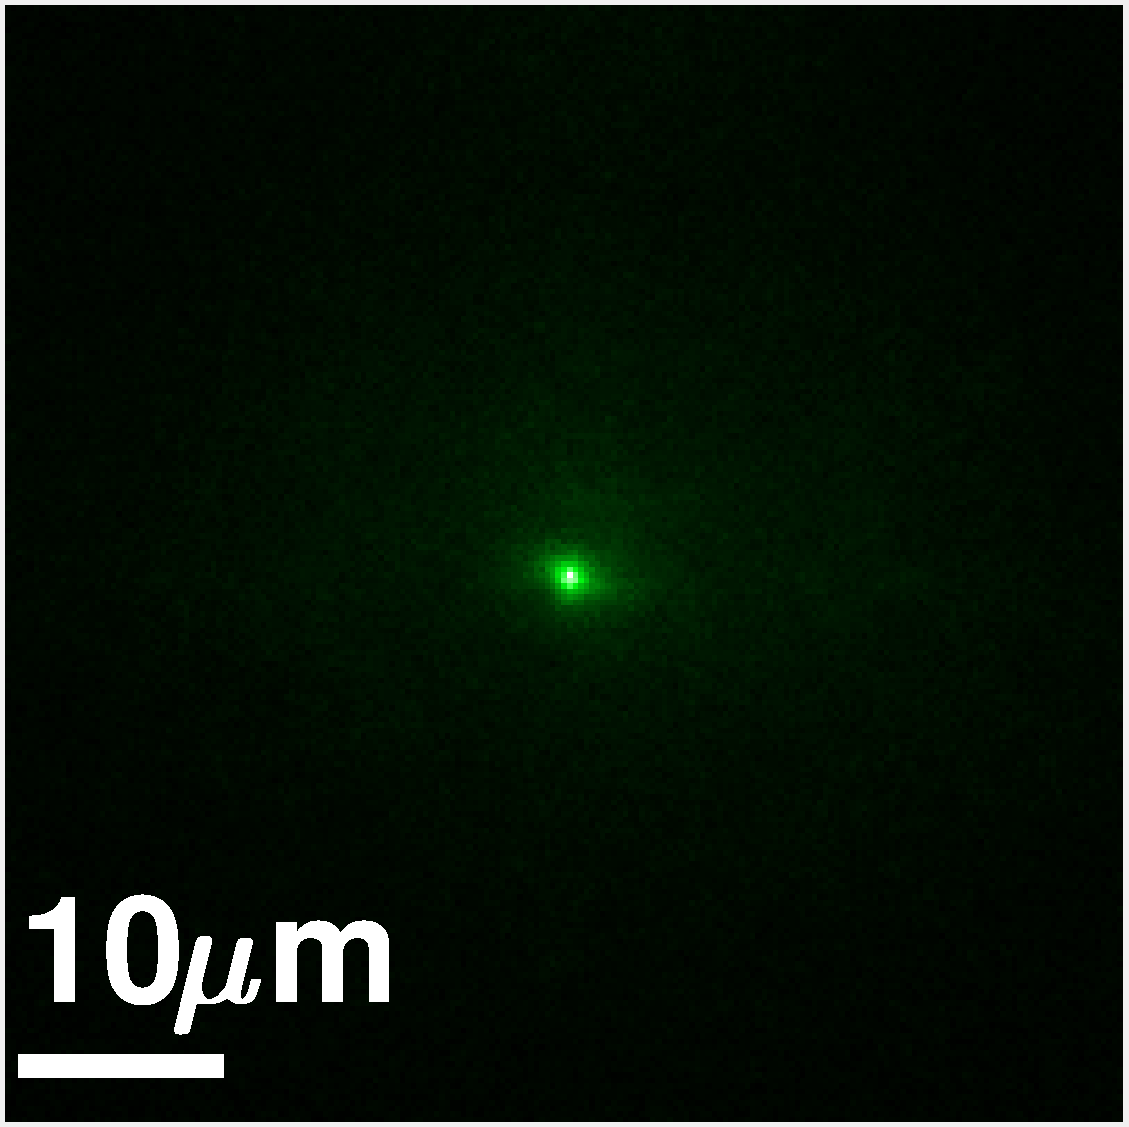
\includegraphics[width = 0.13\textwidth]{figs/confocal_res/fig_converging/2023_01_10_17_18_44/BSI_fin.pdf}&
			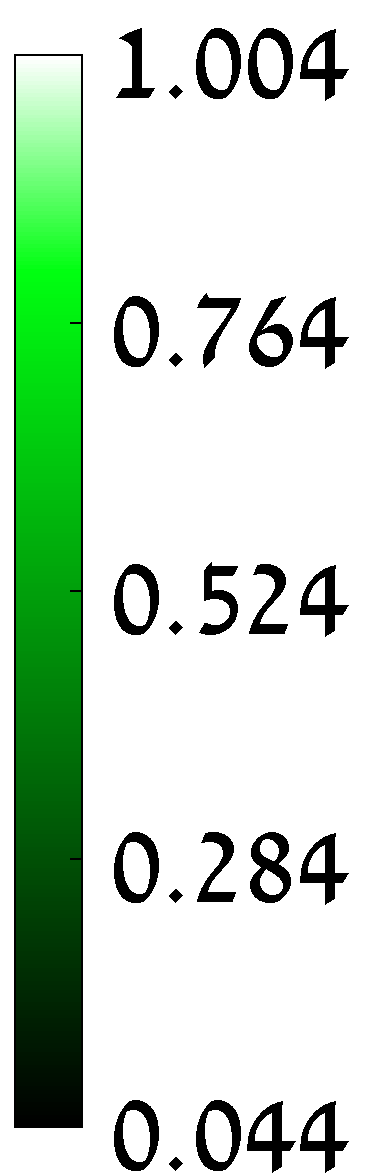
\includegraphics[height = 0.13\textwidth]{figs/confocal_res/fig_converging/2023_01_10_17_18_44/BSI_fin_colorbar.pdf}&
			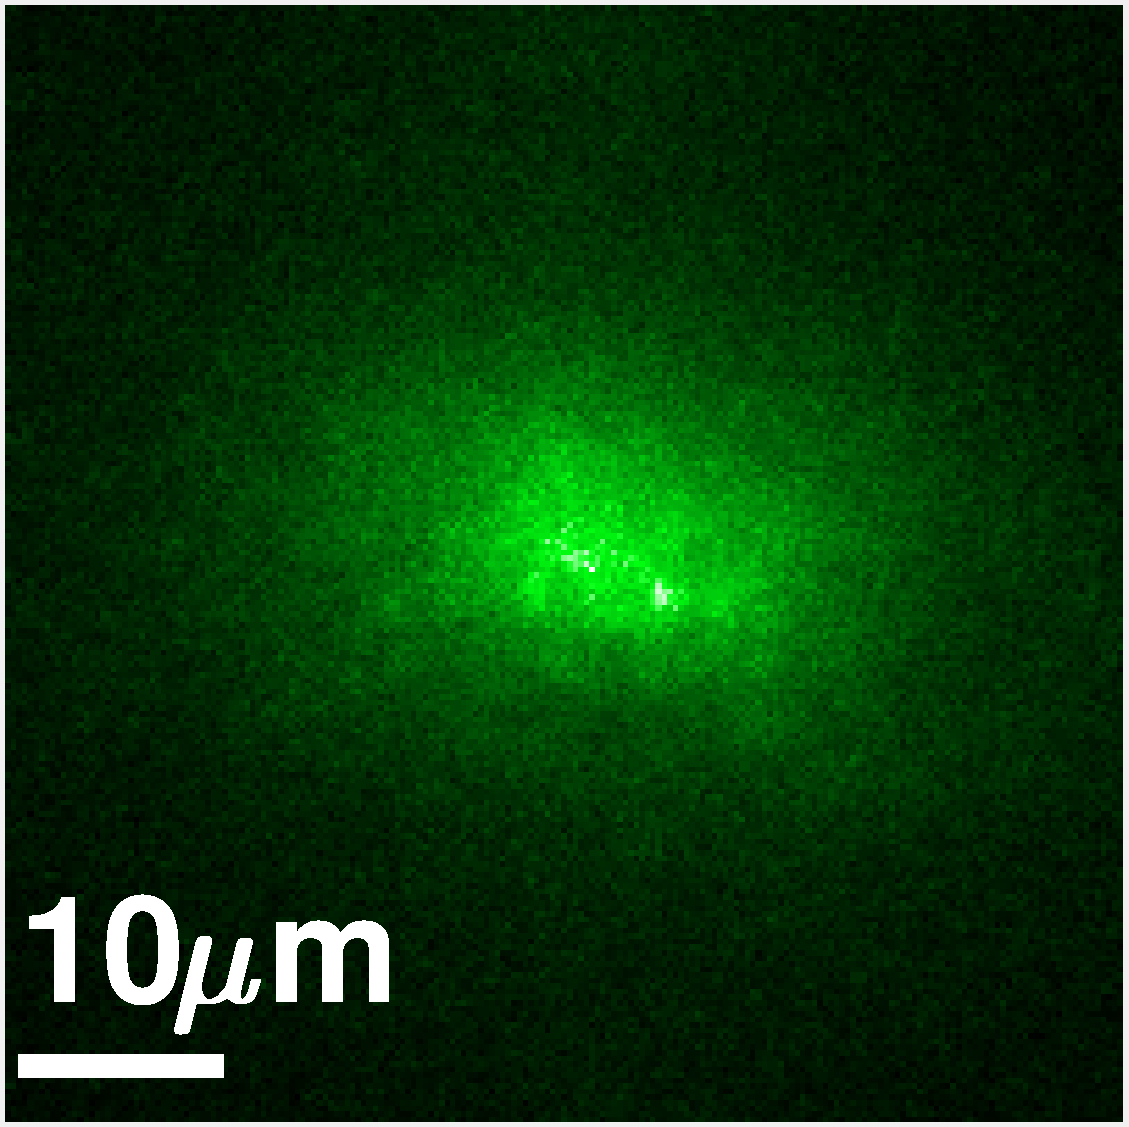
\includegraphics[width = 0.13\textwidth]{figs/confocal_res/fig_converging/2023_01_10_17_18_44/BSI_fin_psf.pdf}&
			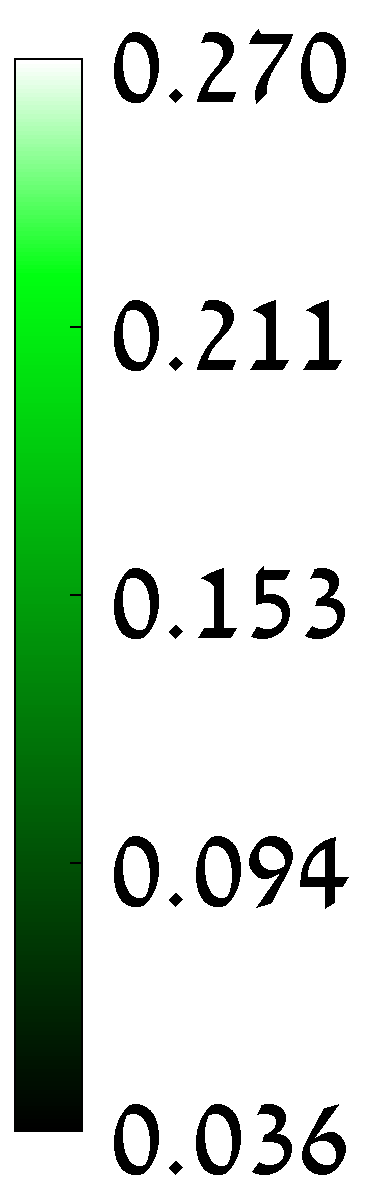
\includegraphics[height = 0.13\textwidth]{figs/confocal_res/fig_converging/2023_01_10_17_18_44/BSI_fin_psf_colorbar.pdf}\\
			
			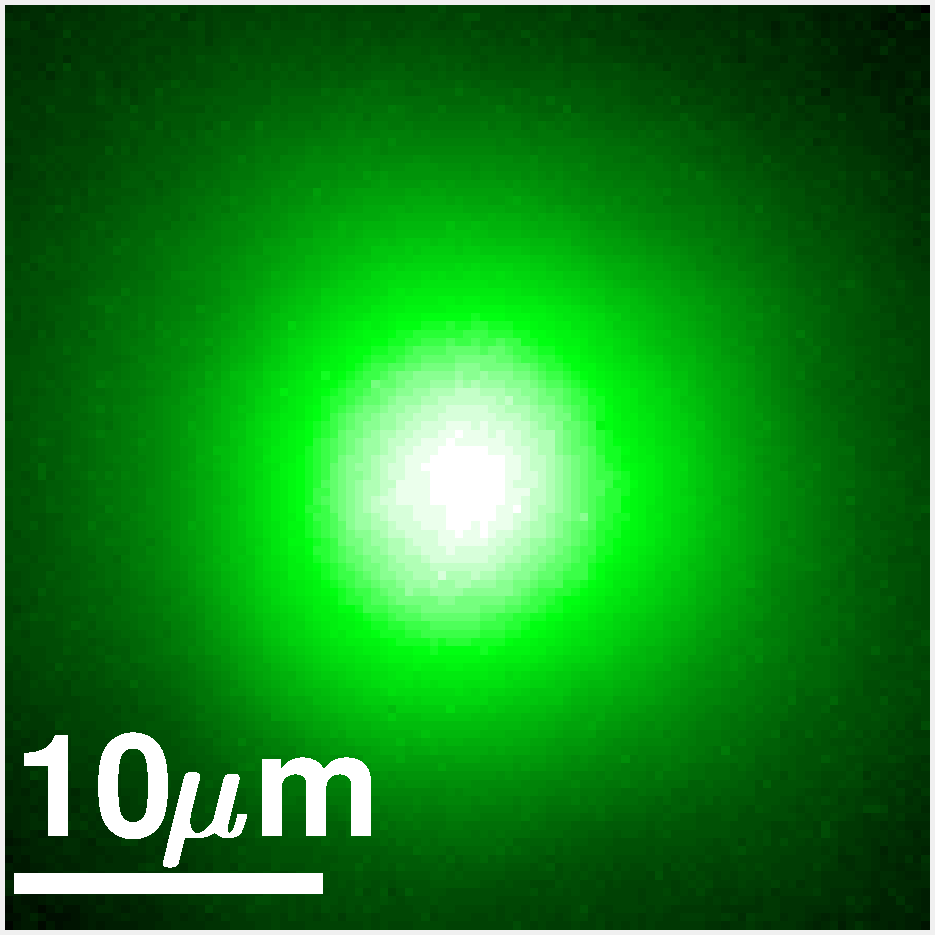
\includegraphics[width= 0.13\textwidth]{figs/confocal_res/fig_big_area/2023_05_16_17_21_45/1.pdf}&
			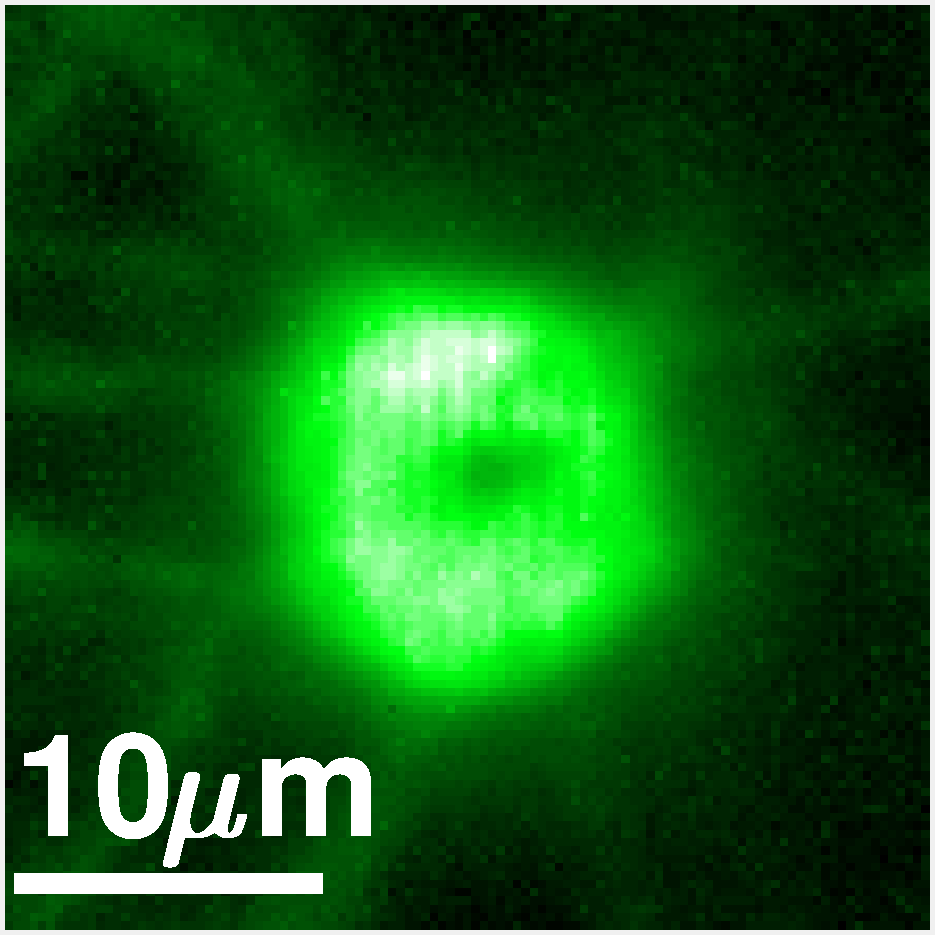
\includegraphics[width= 0.13\textwidth]{figs/confocal_res/fig_big_area/2023_05_16_17_21_45/2.pdf}&
			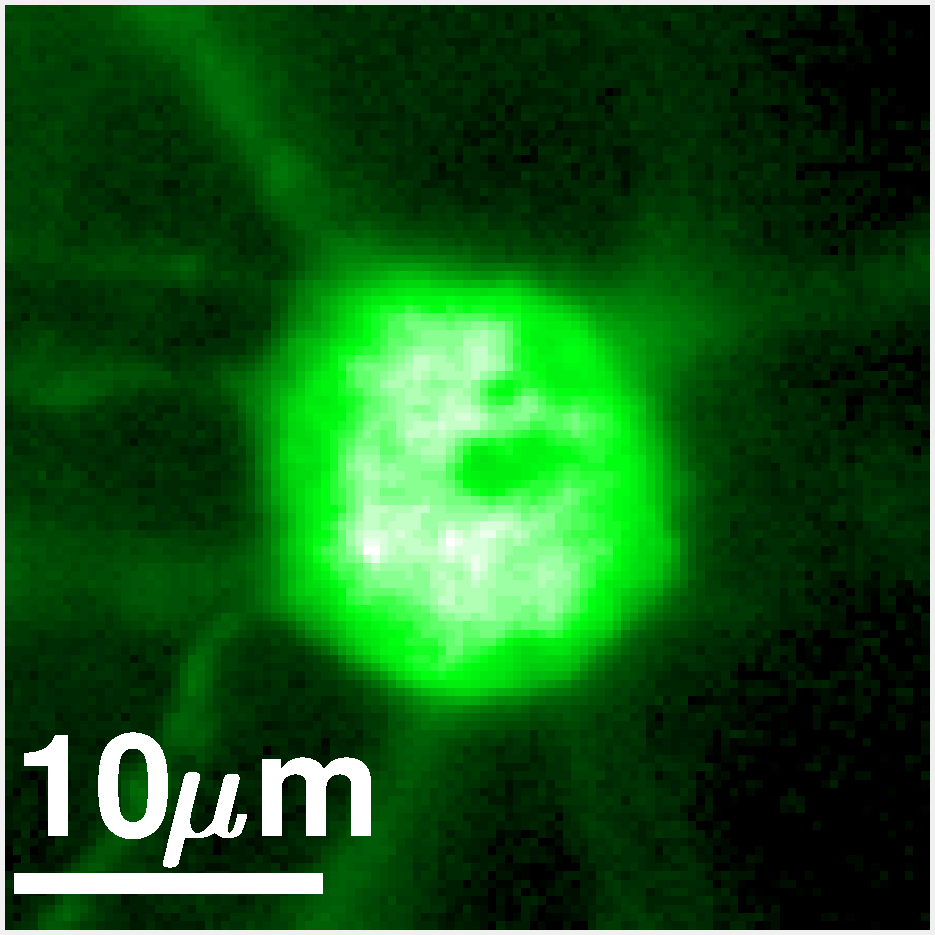
\includegraphics[width= 0.13\textwidth]{figs/confocal_res/fig_big_area/2023_05_16_17_21_45/3.pdf}&
			
				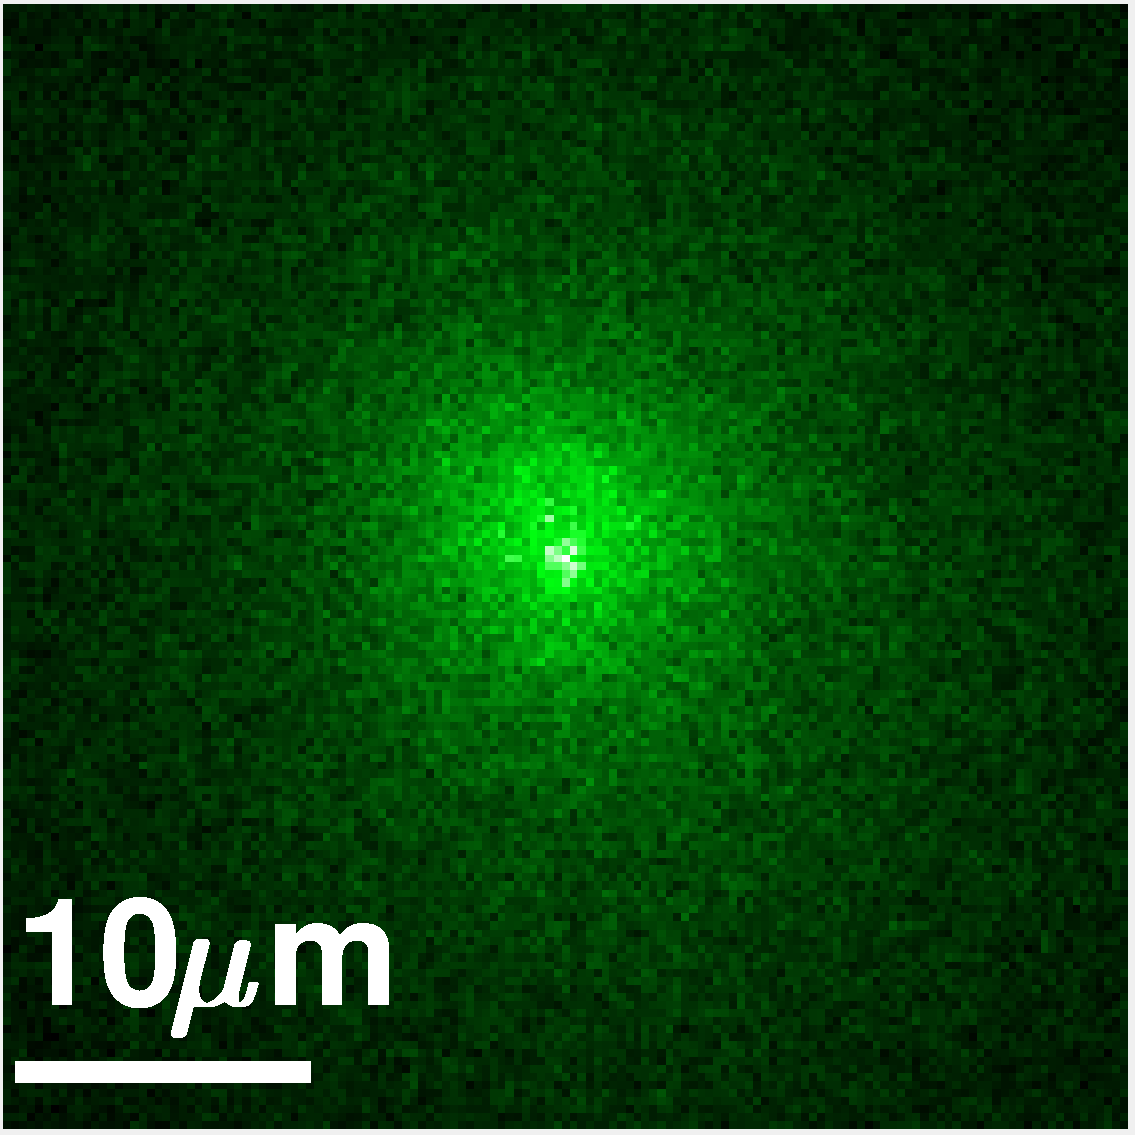
\includegraphics[height = 0.13\textwidth]{figs/confocal_res/fig_converging/4_BSI_init.pdf}&
			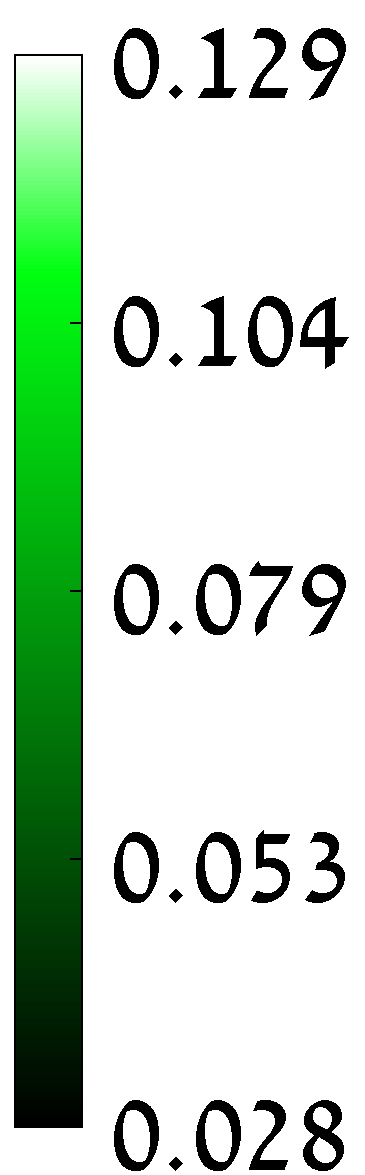
\includegraphics[height = 0.13\textwidth]{figs/confocal_res/fig_converging/4_BSI_init_colorbar.pdf}&
			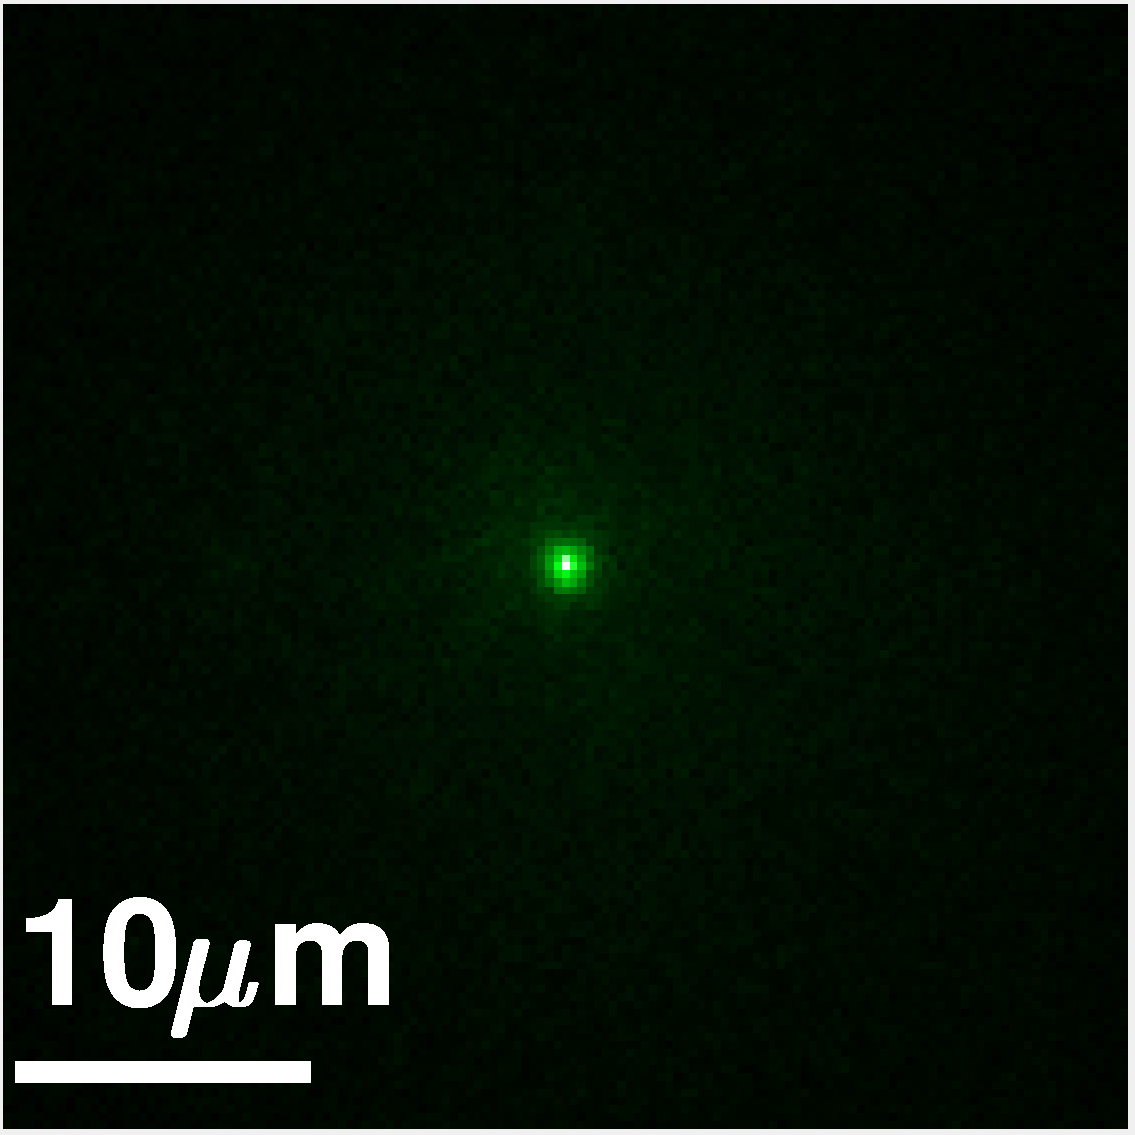
\includegraphics[height = 0.13\textwidth]{figs/confocal_res/fig_converging/4_BSI_fin.pdf}&
			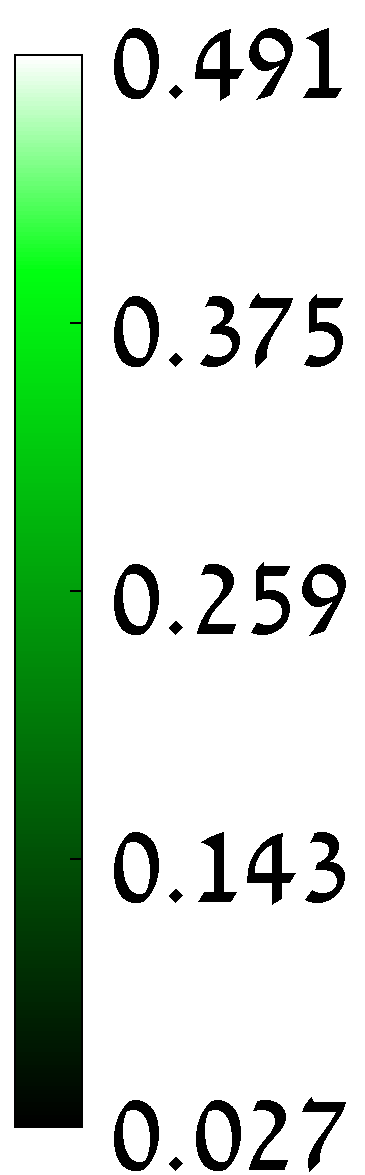
\includegraphics[height = 0.13\textwidth]{figs/confocal_res/fig_converging/4_BSI_fin_colorbar.pdf}&
			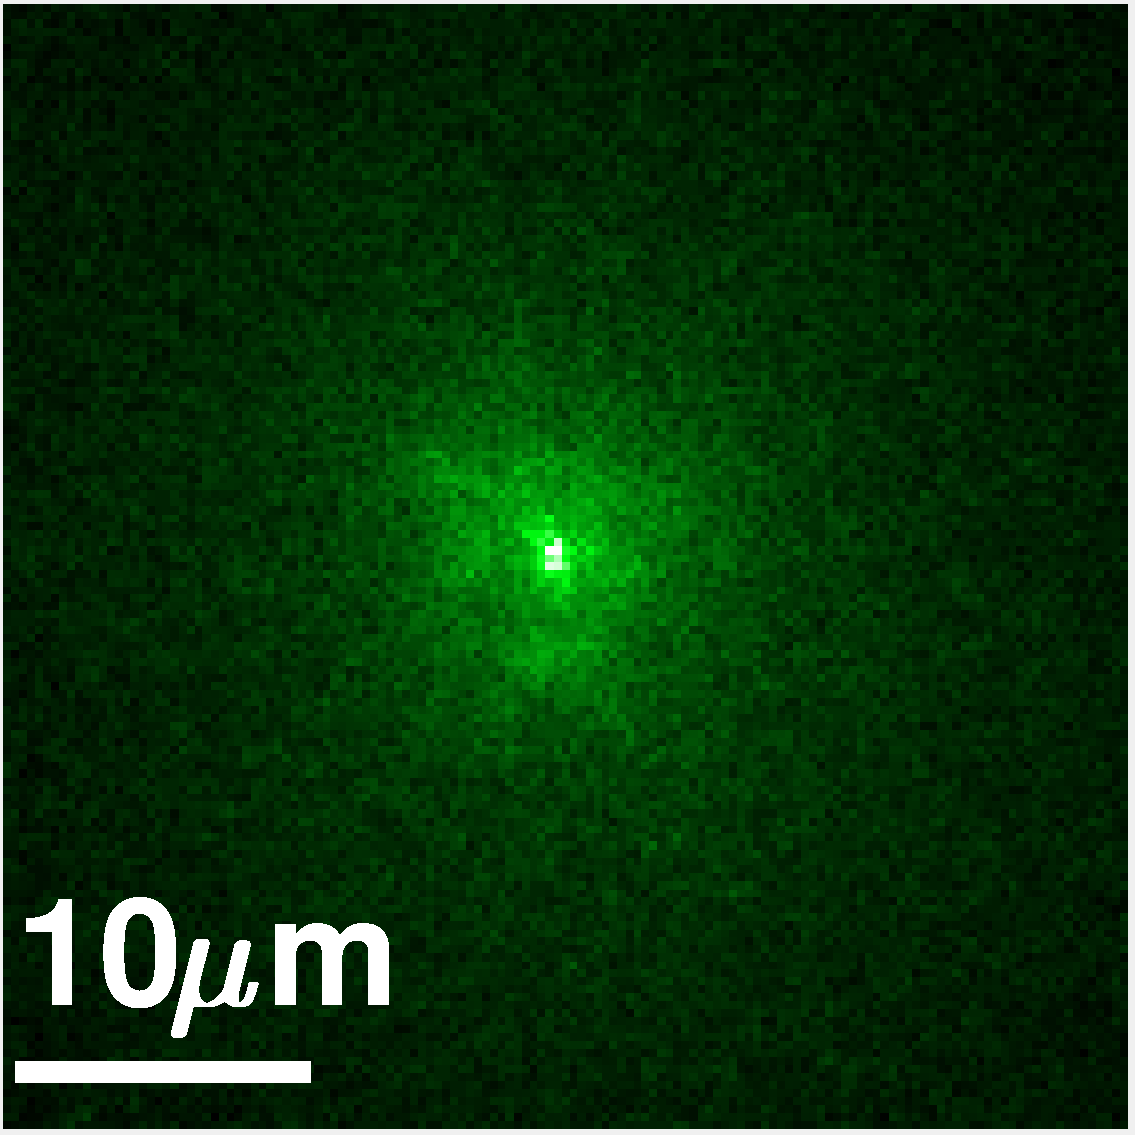
\includegraphics[height = 0.13\textwidth]{figs/confocal_res/fig_converging/4_BSI_fin_psf.pdf}&
			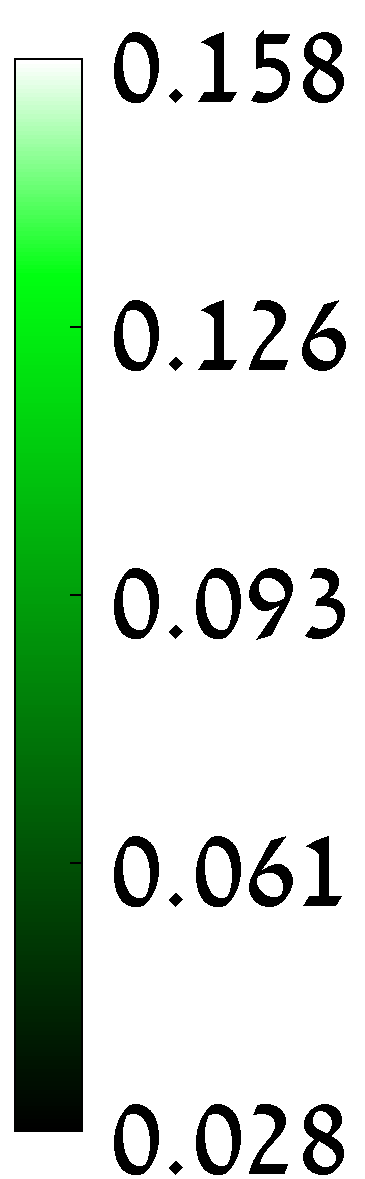
\includegraphics[height = 0.13\textwidth]{figs/confocal_res/fig_converging/4_BSI_fin_psf_colorbar.pdf}\\
					
			{\footnotesize{(a)  w/o mod.}} & {\footnotesize{ (b) w mod. }} & {\footnotesize{ (c) Reference}}  &     		
			\footnotesize{(d) w/o mod.} &   & \footnotesize{(e) w mod.} &   & \footnotesize{(f) PSF} \\
			\multicolumn{3}{c}{\footnotesize{Confocal scan of area}}&\multicolumn{6}{c}{\footnotesize{Single point}}
			
		\end{tabular}
		\caption{{\bf Wavefront shaping results:} Preliminary results of our 1P correction system imaging ex-vivo brain slices.  Left: Confocal scan of the neuron area.    (a) Image of the neuron with no correction, strong scattering is present and the neuron structure is lost. (b) Image with our modulation correction, the neuron shape as well as some of the axons are revealed. (c) A  reference  image of the same neuron. Right: To asses the amount of aberration we also present an image of a single  point. (d) While the objective attempts to focus at a single diffraction limited point, a wide speckle pattern is captured. (e) With modulation on both excitation and emission light we can observe a sharply focused spot. (f) To better asses aberration from one point, we correct only the incoming  light to focus and excite a single point, and measure the resulting scattered pattern
		}\label{fig:confocal-res}
	\end{center}
\end{figure*}


